\section{Numerical Simulations}

\subsection{Stationary single membrane model}
\subsection{Stationary 3 membrane model}
This case deals with a stationary ideal combustion gas separation process with pure methane as fuel. The fuel is mixed with a 20$\%$ oxygen and 5$\%$ carbon dioxide mixture and burned stoichiometric. Note that the percentages refer to the mole percentage of the mixture. The combustion takes place at station 1 in Figure \ref{fig:fig3}. The mole percentages of the reaction products are easy to compute since stoichiometric combustion is assumed. This leads to the following reaction equation:
\begin{align}
	2CH_4 + 4O_2 + 15AR + CO_2 \rightarrow 4H_2O + 3CO_2 + 15AR 
\end{align} 
Directly behind the combustion chamber a condenser is located which will condense all water in the ideal case such that the remaining gas mixture only consists of argon and carbon dioxide. In this case the combustion products are a mixture of 16.667 $\%$ $CO_2$ and 83.333 $\%$ $AR$. This gas mixture is the feed gas stream for station 2 which is a membrane. Stations 3 and 4 represent a membrane as well. \\

The fluid mixture leaving the membranes at the retenate side is feeded back to the previous stage. It is desired that this mixture has the same composition as the original feed. By changing the length of the membrane it is possible to achieve this preference. A longer membrane has a lower concentration of $CO_2$ at the retenate side and a shorter membrane a higher $CO_2$ concentration. The length for each membrane is determined with the single membrane model. Once the length of the membranes are determined the 1 membrane model is extended to the 3 membrane model shown in Figure \ref{fig:fig3}.\\ 
 
The gas mixture leaving the membrane at the permeate side is the feed stream for the next membrane and has a relatively low pressure. To increase the pressure a compressor is placed behind each membrane to enhance gas separation. 

\noindent\begin{minipage}{\linewidth}
	\centering
	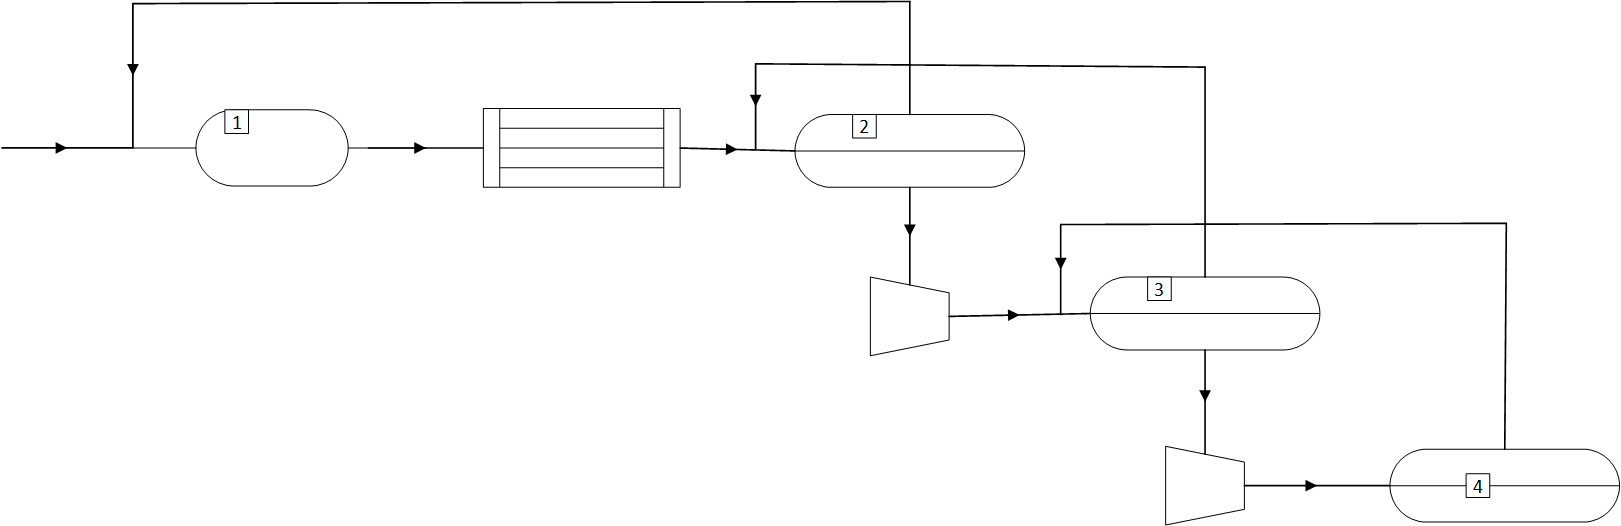
\includegraphics[width= 1\textwidth]{Images/3membranes.png}
	\captionof{figure}{Fluid flow chart 3 membrane model}
	\label{fig:fig3}
	
	\captionof{table}{Fluid flow conditions 3 membrane model}
		\begin{tabular}{|llll|}
		\hline
		Stream no.    &  2        & 3         & 4         \\ \hline
		$L$           &  0.88     & 0.265     & 0.665     \\ \hline
		$\Theta$      & 0.368874  & 0.176977  & 0.800115  \\ \hline
		$P^r $        & 4         & 4         & 4         \\ \hline
		$P^p $        & 0.4       & 0.4       & 0.4       \\ \hline
					  &           &           &   		  \\ \hline		
		$X^{f}_{CO_2}$& 16.666667 & 24.660470 & 60.288259 \\ \hline 
		$X^{f}_{AR}$  & 83.333333 & 75.339530 & 39.711741 \\ \hline 
		$X^{r}_{CO_2}$& 5.000000  & 16.630816 & 24.801102 \\ \hline
		$X^{r}_{AR}$  & 95.000000 & 83.369184 & 75.198898 \\ \hline
		$X^p_{CO_2}$  & 24.660470 & 60.288259 & 73.258709 \\ \hline
		$X^p_{AR}$    & 75.339530 & 39.711741 & 26.641291 \\ \hline
		\end{tabular}
	\label{tab:table2}
\end{minipage} 

\subsection{Transient 3 membrane model}